\documentclass[11pt]{exam}
\usepackage[activeacute,spanish]{babel} % Permite el idioma espa\~nol.
\usepackage[latin1]{inputenc}
\usepackage{amsmath,amsfonts}
\usepackage[colorlinks]{hyperref}
\usepackage{graphicx}

\pagestyle{headandfoot}

\spanishdecimal{.}

\begin{document}

\firstpageheadrule
%\firstpagefootrule
%\firstpagefooter{}{Pagina \thepage\ de \pages}{}
\runningheadrule
%\runningfootrule
\lhead{\bf\normalsize Taller Python 2018}
\rhead{\bf\normalsize Tarea \'area F\'isica}
\cfoot{ }
\lfoot{\tiny GR}
\begin{flushleft}
\vspace{0.2in}
%\hbox to \textwidth{Nombre: \enspace \hrulefill}
%Nombre : \\
\vspace{0.25cm}
\end{flushleft}
%%%%%%%%%%%%%%%%%%%%%%%%%%%%%%%%%%%%%%%%%%

\begin{center}
\textbf{Fecha M'axima de entrega: Viernes 12 de Enero}
\end{center}
\textbf{Instrucciones:} Resuelva el problema propuesto usando Python. Env'ie todos los archivos necesarios para reproducir sus resultados (archivos de datos, c'odigos .py, notebooks .ipynb, etc.) por email a \texttt{grubilar@udec.cl}.

\bigskip

 Una predicci'on de la teor'ia electromagn'etica cl'asica es que una carga el'ectrica $q$ que realiza un movimiento arm'onico simple de la forma
\begin{equation}
\vec{x}(t) = a\cos(\omega_0t)\hat{z},
\end{equation}
emite ondas electromagn'eticas en todas direcciones, en frecuencias $\omega_m$ m'ultiplos  de la frecuencia de oscilaci'on $\omega_0$. En particular, el c'alculo predice que la potencia promedio radiada en la $m-$'esima frecuencia, $\omega_m = m\omega_0$, por unidad de 'angulo s'olido, es dada por la expresi'on
\begin{equation}
\left\langle \frac{dP_{m}}{d\Omega}\right\rangle
=\frac{q^2\mu_0 c}{4\pi}\frac{\omega_0^2m^2}{2\pi}\tan^2\theta\left[ J_{m}\left(\frac{a\omega_0 m}{c}\cos\theta\right)  \right]^2.
\end{equation}
donde $\theta$ es el 'angulo entre la direcci'on de emisi'on y la direcci'on de oscilaci'on de la carga (eje $z$) y $J_m(x)$ es la funci'on de Bessel de primera especie y orden $m$.
\begin{parts}
\item Confeccione un gr'afico coordenadas polares (ver notebook de introducci'on a Matplotlib) que grafique la potencia promedio en funci'on del 'angulo $\theta$, para distintos valores de $m$. El resultado debiese ser algo parecido a lo mostrado en la figura \ref{TER2}
\begin{figure}[ht]
\centerline{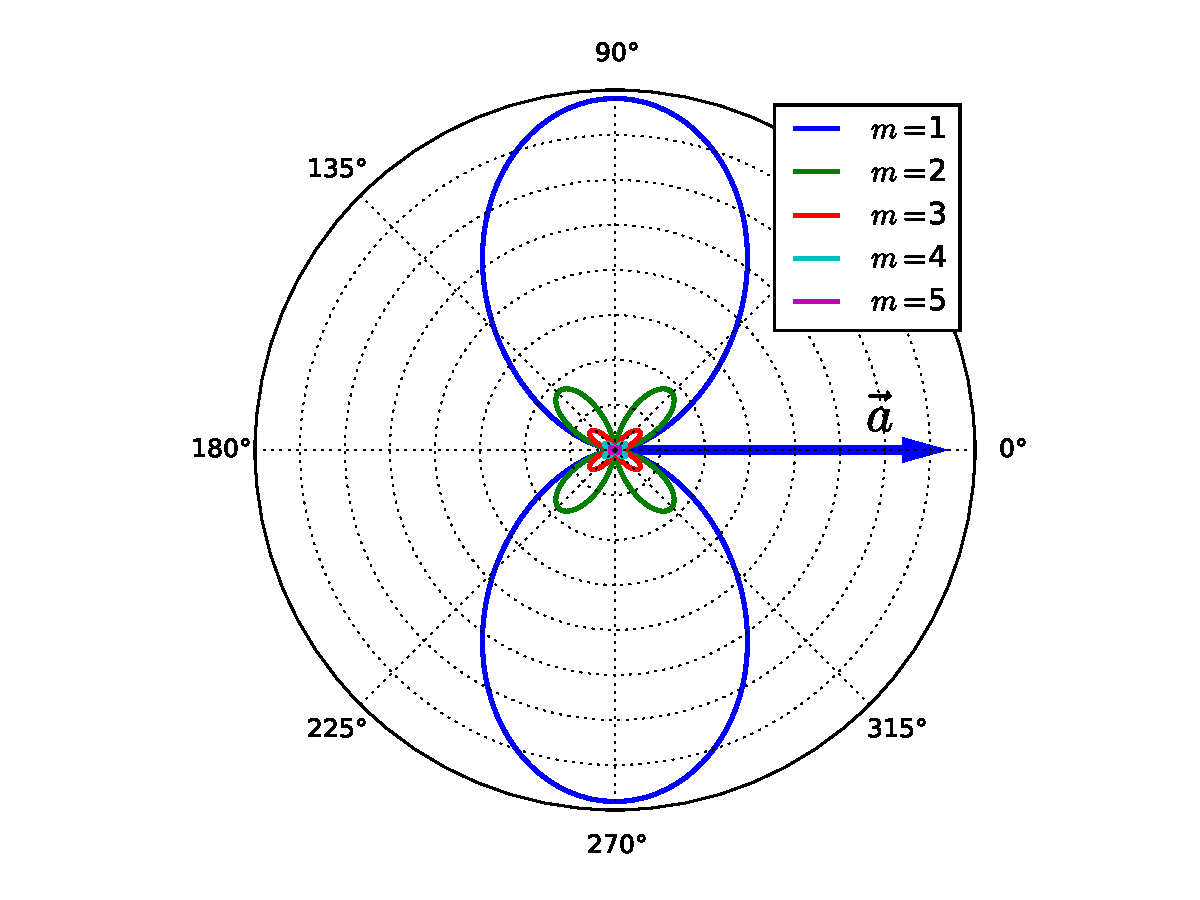
\includegraphics[width=10cm]{figs/fig-mas.pdf}}
\caption{L'obulo de radiaci'on para $m=1,\dots,5$ para $\beta=a\omega_0/c=0.5$.}
\label{TER2}
\end{figure}
\item Evalue (num'ericamente), para $\beta =0.1$ y $\beta = 0.5$ y $m = 1,2,..,5$,  la potencia promedio total radiada, obtenida integrando la expresi'on anterior en todas las direcciones, es decir,
\begin{equation}
\left\langle P_{m}\right\rangle  = \oint\left\langle \frac{dP_{m}}{d\Omega}\right\rangle d\Omega, \quad d\Omega = \sin\theta\,d\theta\,d\varphi.
\end{equation}
Imprima los valores obtenidos y graf'iquelos, para obtener un resultado similar al mostrado en la figura \ref{TER3}.
\begin{figure}[ht]
\centerline{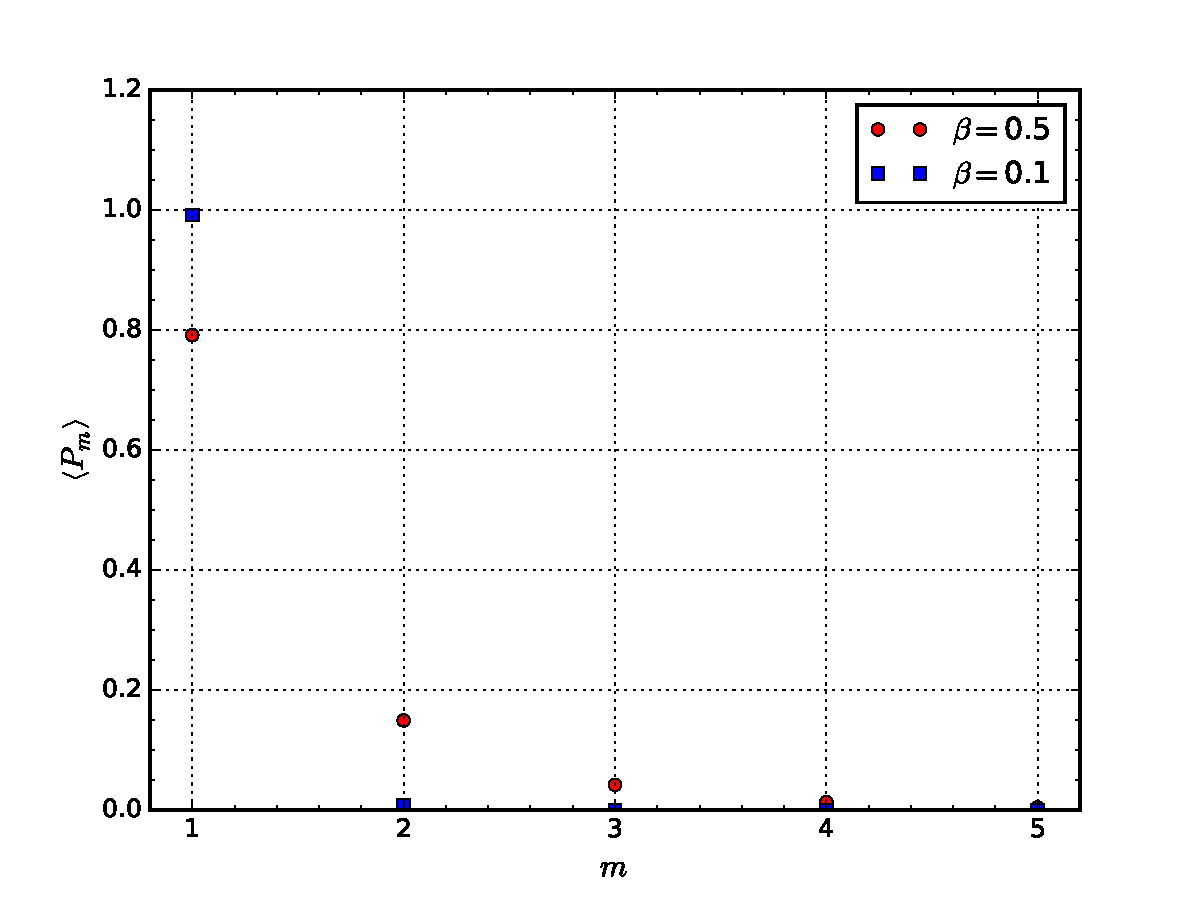
\includegraphics[width=10cm]{figs/fig-mas-potencia-total-comparacion.pdf}}
 \caption{Potencia promedio radiada para $m=1,\cdots,5$, con par'ametros de velocidad $\beta=0.5$ y  $\beta=0.1$, normalizadas respecto a la potencia total.}
\label{TER3}
\end{figure}
\end{parts}
\end{document} 
